\chapter{Preliminaries}

\section{Terminology and Conventions}

To ensure clarity and consistency throughout this report, the following standardized terminology and capitalization conventions are utilized:

\begin{longtable}{llp{8cm}}
\caption{Standardized Technical Terminology} \label{tab:terminology} \\
\toprule
\textbf{Term} & \textbf{Capitalization} & \textbf{Description / Usage} \\
\midrule
\endfirsthead
\multicolumn{3}{c}{\textit{Standardized Technical Terminology (continued)}} \\
\toprule
\textbf{Term} & \textbf{Capitalization} & \textbf{Description / Usage} \\
\midrule
\endhead
\midrule \multicolumn{3}{r}{\textit{(continued on next page)}} \\
\endfoot
\bottomrule
\endlastfoot
\textbf{Vector Database} & Capitalized & The high-dimensional similarity search engine (e.g., Qdrant) used for dense retrieval. \\
\textbf{BM25} & All Caps & The probabilistic lexical ranking function used for keyword-based sparse retrieval. \\
\textbf{RAG} & All Caps & Retrieval-Augmented Generation; the core system architecture. \\
\textbf{MRAG} & All Caps & Multimodal Retrieval-Augmented Generation; the specialized extension of RAG for handling non-textual data. \\
\textbf{LLM} & All Caps & Large Language Model (e.g., GPT-4o-mini, Claude 3.5 Sonnet). \\
\textbf{Multimodal} & Sentence Case & Systems or processes involving multiple data modalities (text, image, audio, video). \\
\textbf{ASR} & All Caps & Automatic Speech Recognition; the technology used to transcribe audio/video lecture content. \\
\textbf{OCR} & All Caps & Optical Character Recognition; the process of extracting text from rasterized document images. \\
\textbf{VLM} & All Caps & Vision-Language Model; models that process both visual and textual inputs (e.g., ColQwen, SmolVLM). \\
\textbf{Docling} & Title Case & The specialized document parsing library used for structural extraction. \\
\textbf{ColQwen} & Title Case & The vision-language model architecture used for visual document retrieval. \\
\textbf{Hybrid Search} & Capitalized & The combination of sparse (BM25) and dense (Vector) retrieval pathways. \\
\textbf{RRF} / \textbf{DBSF} & All Caps & Reciprocal Rank Fusion and Distribution-Based Score Fusion (fusion algorithms). \\
\textbf{FAISS} & All Caps & Facebook AI Similarity Search; a library for fast similarity search and clustering of embeddings. \\
\textbf{HNSW} & All Caps & Hierarchical Navigable Small World; an efficient similarity search algorithm used in vector indices. \\
\textbf{nDCG} & Notation & Normalized Discounted Cumulative Gain; an information retrieval metric for evaluating ranking quality. \\
\textbf{MaxSim} & Notation & Maximum Similarity; the token-level scoring mechanism used in late-interaction models like ColBERT. \\
\textbf{ColBERT} & Title Case & Contextualized Late Interaction over BERT; a dense retrieval architecture using token-level interactions. \\
\textbf{AWS} & All Caps & Amazon Web Services; the cloud platform used for deployment and infrastructure. \\
\textbf{S3} & All Caps & Amazon Simple Storage Service; object storage service for document artifacts and processing outputs. \\
\textbf{ECS} & All Caps & Amazon Elastic Container Service; container orchestration service for running the BK-MInD application. \\
\textbf{SageMaker} & Title Case & AWS SageMaker; machine learning service used for model hosting and inference scaling. \\
\textbf{WAF} & All Caps & Web Application Firewall; AWS WAF provides protection against application-level attacks. \\
\textbf{JWT} & All Caps & JSON Web Token; cryptographic token used for authenticating API requests. \\
\textbf{TLS} & All Caps & Transport Layer Security; encryption protocol for securing data in transit. \\
\textbf{SSE} & All Caps & Server-Side Encryption; encryption method for protecting data at rest in Amazon S3. \\
\textbf{API} & All Caps & Application Programming Interface; the interface through which frontend and backend systems communicate. \\
\textbf{REST} & All Caps & Representational State Transfer; architectural style for the backend API design. \\
\textbf{SRT} & All Caps & SubRip Text; subtitle file format used for storing transcription outputs. \\
\textbf{VTT} & All Caps & Web Video Text Tracks; subtitle file format used for web-based video player integration. \\
\textbf{DPI} & All Caps & Dots Per Inch; resolution parameter used when rasterizing PDF pages to images. \\
\textbf{CI/CD} & All Caps & Continuous Integration / Continuous Deployment; automated pipeline for testing and deployment. \\
\end{longtable}

\section{Automatic Speech Recognition}
\label{sec:asr}

Automatic Speech Recognition (ASR) converts spoken language into text. It has evolved from statistical pipelines to end-to-end neural models and is widely used in transcription, captioning, accessibility, and voice interfaces~\cite{graves2006ctc, chan2015las}. Recent work emphasizes robustness, low-resource languages, and large-scale pretraining~\cite{baevski2020wav2vec2, radford2022whisper}. A typical ASR pipeline is illustrated in Figure~\ref{fig:ASR_Pipeline}\footnote{\url{https://www.researchgate.net/figure/ASR-application-pipeline_fig1_355070202}}.

\begin{figure}[H]
    \centering
    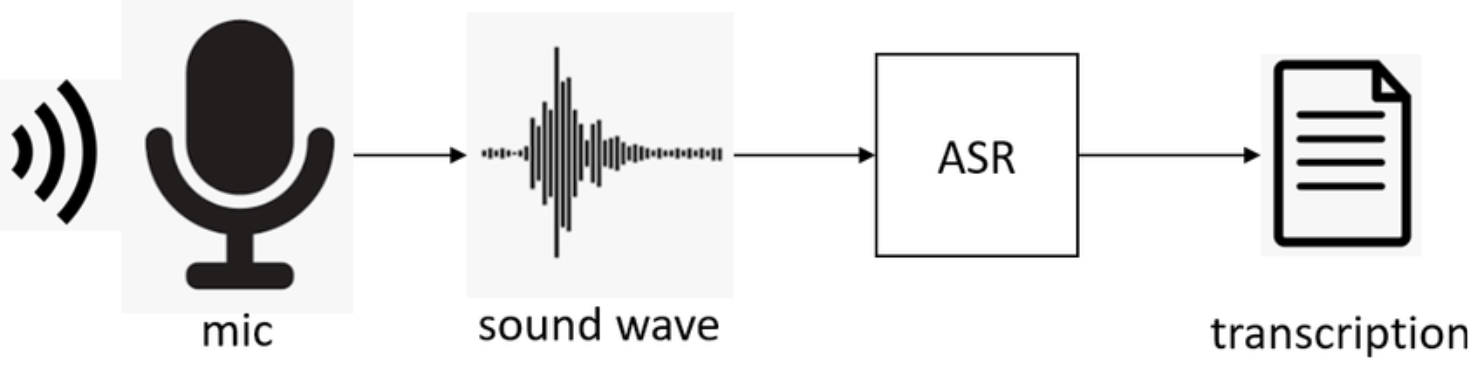
\includegraphics[width=0.9\textwidth]{img/pdz/09-asr-pipeline.png}
    \caption[ASR pipeline]{ASR pipeline}
    \label{fig:ASR_Pipeline}
\end{figure}

ASR is the task of converting an acoustic signal into a sequence of words. Formally, the goal of an ASR system is to determine the most probable word sequence $\hat{W}$ given an input acoustic observation $X$

\begin{equation*}
    \hat{W} = \arg\max_{W} P(W|X).
\end{equation*}

Using Bayes' theorem, this can be rewritten as

\begin{equation*}
    \hat{W} = \arg\max_{W} P(X|W)P(W)
\end{equation*}

where
\begin{itemize}
    \item $P(X|W)$ is the \textbf{acoustic model}, representing the probability of observing the audio features given a word sequence;
    \item $P(W)$ is the \textbf{language model}, representing the prior probability of a word sequence in the target language;
    \item $\hat{W}$ is the final predicted transcription.
\end{itemize}

The decoder combines the acoustic and language models to search for the optimal word sequence that maximizes this probability.


Early ASR systems used Gaussian Mixture Models with Hidden Markov Models (GMM--HMMs) for acoustic modeling and temporal alignment~\cite{hinton2012dnn, rabiner1989hmm}. Later DNN--HMM hybrids replaced GMM acoustic models with neural networks and became common in production systems, supported by toolkits such as Kaldi~\cite{povey2011kaldi} and benchmarks such as Switchboard and WSJ~\cite{switchboard1992, wsj1993}.

End-to-end ASR directly maps audio to text with a single neural model. The main paradigms are CTC, which removes the need for frame-level alignments~\cite{graves2006ctc}; attention-based encoder--decoder models such as LAS, which model output dependencies through attention~\cite{chan2015las}; and transducer models such as RNN-T, which support streaming and low-latency inference~\cite{graves2012rnnt, he2019transformertransducer}.

End-to-End ASR using Connectionist Temporal Classification (CTC) models the probability of a label sequence $Y$ by summing over all possible alignments $\pi$ that collapse to $Y$

\begin{equation*}
    P(Y|X) = \sum_{\pi \in \mathcal{B}^{-1}(Y)} P(\pi|X)
\end{equation*}

where $\mathcal{B}$ is the mapping that removes blanks and repeated labels from the alignment path.


Transformers further improved ASR through global self-attention. Conformer augments Transformers with convolutional modules to capture local acoustic patterns while preserving global context, achieving strong results on benchmarks such as LibriSpeech~\cite{gulati2020conformer, panayotov2015librispeech}.

In attention-based ASR models, the system generates the output transcription autoregressively, producing one token at a time conditioned on previous outputs and the encoded acoustic features. The probability of generating a transcription sequence $Y$ given the input speech features $X$ is formulated as

\begin{equation*}
    P(Y|X) = \prod_{t=1}^{T} P(y_t \mid y_{1:t-1}, X)
\end{equation*}

where
\begin{itemize}
    \item $X$ is the input acoustic feature sequence extracted from the speech signal;
    \item $Y = (y_1, y_2, \dots, y_T)$ is the output sequence of tokens (e.g., characters, subwords, or words);
    \item $y_t$ is the token predicted at timestep $t$;
    \item $y_{1:t-1}$ denotes all previously generated tokens before timestep $t$;
    \item $T$ is the length of the output sequence;
    \item $P(y_t \mid y_{1:t-1}, X)$ is the conditional probability of generating token $y_t$ given the input features and prior predictions.
\end{itemize}

The decoder uses an attention mechanism to dynamically focus on relevant parts of the encoded speech representation at each timestep, enabling the model to learn soft alignments between acoustic frames and output tokens without explicit alignment labels.

Self-supervised pretraining is another major direction. Models such as wav2vec 2.0 learn from unlabeled audio and can be fine-tuned with limited labels, while Whisper shows that scaling data and model size improves robustness and multilingual transfer.

ASR evaluation commonly uses LibriSpeech~\cite{panayotov2015librispeech}, Switchboard~\cite{switchboard1992}, TED-LIUM~\cite{rousseau2012tedlium}, and Common Voice~\cite{ardila2020commonvoice}. The main metrics are Word Error Rate (WER) and Character Error Rate (CER).

These metrics measure the difference between the reference transcription and the hypothesis transcription produced by the system. Word Error Rate (WER) is computed as

\begin{equation*}
    \text{WER} = \frac{S + D + I}{N}
    \label{eq:wer}
\end{equation*}

where
\begin{itemize}
    \item $S$ is the number of word substitutions;
    \item $D$ is the number of word deletions;
    \item $I$ is the number of word insertions;
    \item $N$ is the total number of words in the reference transcript.
\end{itemize}

Character Error Rate (CER) applies the same formulation at the character level:

\begin{equation}
    \text{CER} = \frac{S + D + I}{N}
    \label{eq:cer}
\end{equation}

where $S$, $D$, and $I$ are the number of character substitutions, deletions, and insertions, respectively, and $N$ is the total number of reference characters.

Lower WER and CER values indicate better recognition performance, with $\text{WER} = 0$ and $\text{CER} = 0$ representing perfect transcriptions.

Practical ASR still faces challenges in noise, accents, domain shifts, streaming latency, and on-device constraints. Current research therefore focuses on multilingual and code-switching recognition, efficient streaming architectures, model compression, diarization, alignment, and confidence estimation for safer deployment.


\section{Optical Character Recognition}
\label{sec:ocr}

Optical Character Recognition (OCR) extracts text from scanned documents and images. It has progressed from rule-based and template-matching methods to deep learning systems that support digitization, automation, and document understanding across many domains \cite{smith2007tesseract, chen2021textrecognition}.

\begin{figure}[H]
    \centering
    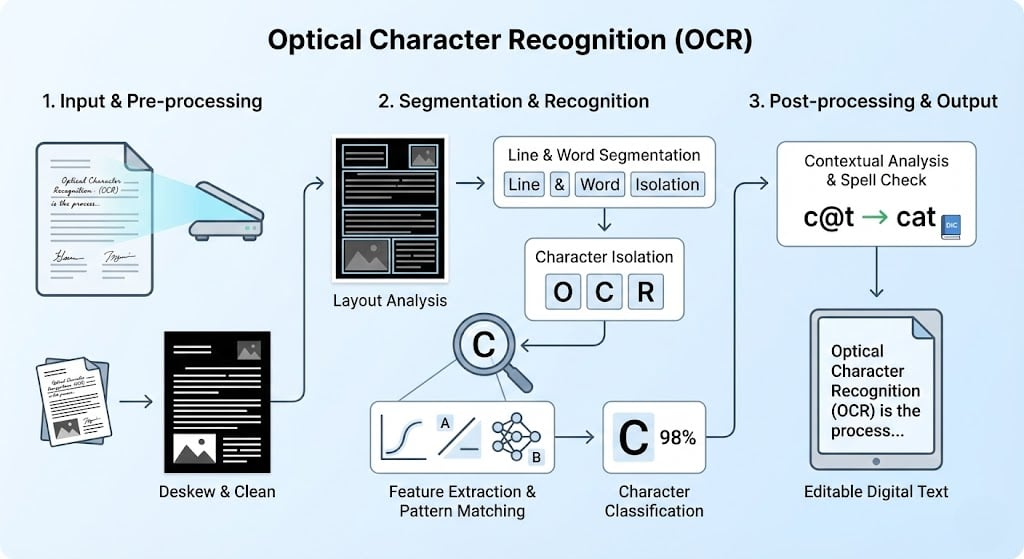
\includegraphics[width=0.9\textwidth]{img/pdz/10-ocr-pipeline.jpg}
    \caption[OCR Pipeline]{OCR pipeline.}
    \label{fig:OCR pipeline}
\end{figure}

Early OCR systems relied on mechanical recognition and template matching, which worked only in constrained settings and were sensitive to fonts, noise, and document quality \cite{govindaraju1993handwritten}. Commercial use expanded in banking and postal services, but robustness remained limited \cite{mori1992historical}.

Conventional OCR pipelines used segmentation, feature extraction, and classification. Hand-crafted features such as zoning, projection profiles, and contours were paired with classifiers such as SVMs and HMMs \cite{casey1996survey}. Handwriting remained harder because of style variation, cursiveness, and ligatures, motivating more flexible statistical approaches \cite{plamondon2000handwriting}.

Deep learning transformed OCR by replacing hand-crafted features with learned visual and sequence representations. CNNs learn spatial features directly from images \cite{lecun1998gradient}, while RNN/LSTM models and CTC support sequence recognition without explicit character segmentation \cite{graves2009novel, graves2006ctc}. More recently, transformer-based systems such as TrOCR have improved recognition across scripts and visual conditions \cite{li2023trocr}.

With advances in deep learning, end-to-end models such as CRNN and Transformer-based architectures directly learn visual-to-text mappings from raw images \cite{shi2016crnn, baek2019whatiswrong, li2021trocr}. These models estimate the output text sequence by maximizing the conditional probability given the input image

\begin{equation*}
    \hat{Y} = \arg\max_{Y} P(Y|X)
\end{equation*}

where $X$ denotes the input image and $Y$ is the predicted text sequence.

Although OCR has improved significantly, handwritten documents, low-resolution images, multilingual text, domain-specific noise, and complex page layouts remain difficult. OCR is commonly evaluated using Character Error Rate (CER) and Word Error Rate (WER), following the same edit-distance formulation defined in Section~\ref{sec:asr}, Equations~\ref{eq:cer} and~\ref{eq:wer}. Lower CER and WER indicate better recognition performance.

Scene text recognition (STR) extends OCR to text in natural images, where backgrounds, distortion, and lighting are uncontrolled. Modern STR often combines object detection models such as Faster R-CNN or YOLO with recognition modules to improve text localization and transcription \cite{baek2019whatiswrong}.

OCR supports archive digitization \cite{holley2009howgood}, check and identity-document processing \cite{govindaraju1994handwritten}, medical record digitization \cite{zhou2022automatic}, assistive reading technologies \cite{anagnostopoulos2006license}, and license plate recognition \cite{du2013automatic}.

Key research directions include self-supervised learning to reduce labeled-data dependence, multimodal OCR that combines visual and linguistic cues, and few-shot methods for underrepresented languages and scripts \cite{li2023trocr}. Overall, OCR bridges visual and textual information and remains central to document automation and accessibility.

\section{Transformer}
\label{sec:transformer}
The Transformer model described in this section is based on \emph{Attention Is All You Need}~\cite{vaswani2017attention}. It replaces recurrent sequence processing with self-attention, enabling parallel training and effective modeling of long-range dependencies in tasks such as translation, generation, and language understanding.

\begin{figure}[H]
    \centering
    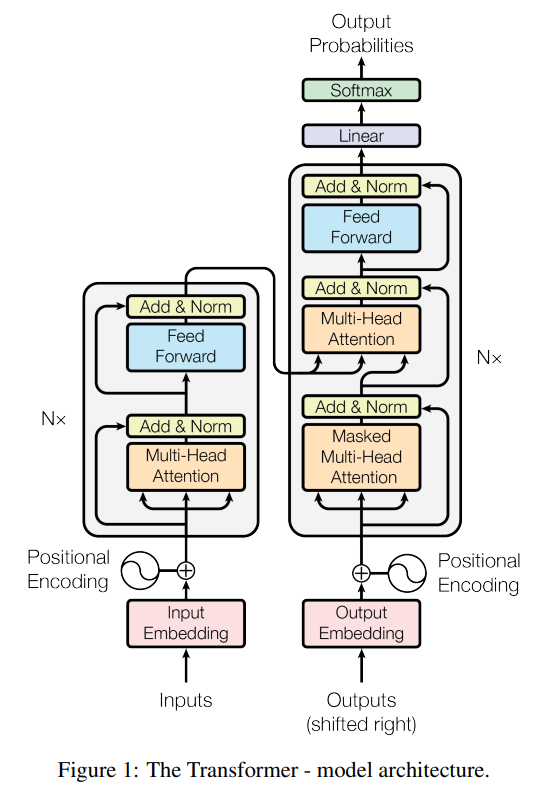
\includegraphics[width=0.5\textwidth]{img/pdz/06-transformers-architecture.png}
    \caption[Transformer Architecture]{Transformer Architecture.}
    \label{fig:Transformer architecture}
\end{figure}

A Transformer consists of an \textbf{Encoder} and a \textbf{Decoder}, each composed of $N$ identical layers ($N = 6$ in the original implementation).

Each Encoder layer contains two sub-layers:
\begin{enumerate}
    \item Multi-head self-attention.
    \item Position-wise fully connected feed-forward network.
\end{enumerate}
Each sub-layer is wrapped with a residual connection. The output of each sub-layer is
\[
\mathrm{LayerNorm}(x + \mathrm{Sublayer}(x)).
\]

Each Decoder layer contains three sub-layers:
\begin{enumerate}
    \item Masked multi-head self-attention, preventing each position from attending to future tokens.
    \item Multi-head attention over the Encoder outputs.
    \item Position-wise feed-forward network.
\end{enumerate}
As in the Encoder, residual connections and layer normalization are applied to each sub-layer.

Because the Transformer contains no recurrence or convolution, positional information must be injected explicitly. The model adds Positional Encodings to input embeddings at the bottoms of both the Encoder and Decoder stacks. The original Transformer uses sinusoidal encodings defined as
\[
\mathrm{PE}(pos, 2i) = \sin\left(\frac{pos}{10000^{2i / d_{\text{model}}}}\right),
\]
\[
\mathrm{PE}(pos, 2i+1) = \cos\left(\frac{pos}{10000^{2i / d_{\text{model}}}}\right),
\]
where $pos$ is the token position and $i$ is the dimension index. Each dimension corresponds to a sinusoid at a different frequency, enabling the model to encode both absolute and relative positional patterns.

Self-attention computes an output for each position by mapping a query vector to a set of key-value pairs.


Similarity between queries and keys is computed via the dot product $QK^{T}$, followed by a softmax to obtain attention weights. Because large values can destabilize gradients when the dimensionality $d_{K}$ is high, the dot products are scaled by $\sqrt{d_{K}}$
\begin{equation}
\label{eq:attention}
\mathrm{Attention}(Q, K, V)
= \mathrm{softmax}\left( \frac{QK^{T}}{\sqrt{d_{K}}} \right) V.
\end{equation}

where
\begin{itemize}
    \item $Q \in \mathbb{R}^{T_q \times d}$ are query vectors representing what information to look for;
    \item $K \in \mathbb{R}^{T_k \times d}$ are key vectors representing what information is available;
    \item $V \in \mathbb{R}^{T_k \times d}$ are value vectors containing the actual information to be extracted;
    \item $d_K$ (or $d$) is the dimension of the key/query vectors;
    \item $T_q, T_k$ are the sequence lengths for queries and keys respectively.
\end{itemize}

Instead of performing a single attention operation, the Transformer projects queries, keys, and values into $h$ subspaces using learned linear transformations. Attention is computed independently in each head
\[
\text{head}_{i} = \mathrm{Attention}(QW_i^{Q},\, KW_i^{K},\, VW_i^{V}).
\]
The outputs of all $h$ heads are concatenated and linearly transformed
\[
\mathrm{MultiHead}(Q,K,V) = 
\mathrm{Concat}(\text{head}_1, \ldots, \text{head}_h) W^{O}.
\]

This mechanism allows the model to capture multiple types of relationships simultaneously by attending to diverse representation subspaces.


\section{Multimodal Fusion and Cross-Attentional Models}

Specialized retrieval pipelines often need to combine visual, audio, motion, and ASR-text signals rather than relying on a single encoder. For video retrieval, M2HF uses multi-stream feature extraction, attentional fusion, and multi-level feature/decision fusion to produce richer retrieval signals~\cite{liu2022m2hf}.

Cross-attentional models are especially useful for reranking. Unlike dual encoders, cross-encoders jointly process the query and document, allowing token-level interactions that capture fine semantic distinctions. This improves precision but is computationally expensive, so cross-attention is usually applied to a smaller candidate set after first-stage retrieval~\cite{zhu2024reranking, yoo2021cooperative}\footnote{\url{https://www.pinecone.io/learn/series/rag/rerankers/}}. 

Cross-attention computes attention weights using queries from one sequence and key-value pairs from another. Given query matrix $Q$, key matrix $K$, and value matrix $V$

\begin{equation*}
    \text{Attention}(Q, K, V) = \text{softmax}\left(\frac{QK^{T}}{\sqrt{d_k}}\right)V
\end{equation*}

The cross-attention mechanism is illustrated in Figure~\ref{fig:Cross-attention}\footnote{\url{https://magazine.sebastianraschka.com/p/understanding-multimodal-llms}}.

\begin{figure}[H]
    \centering
    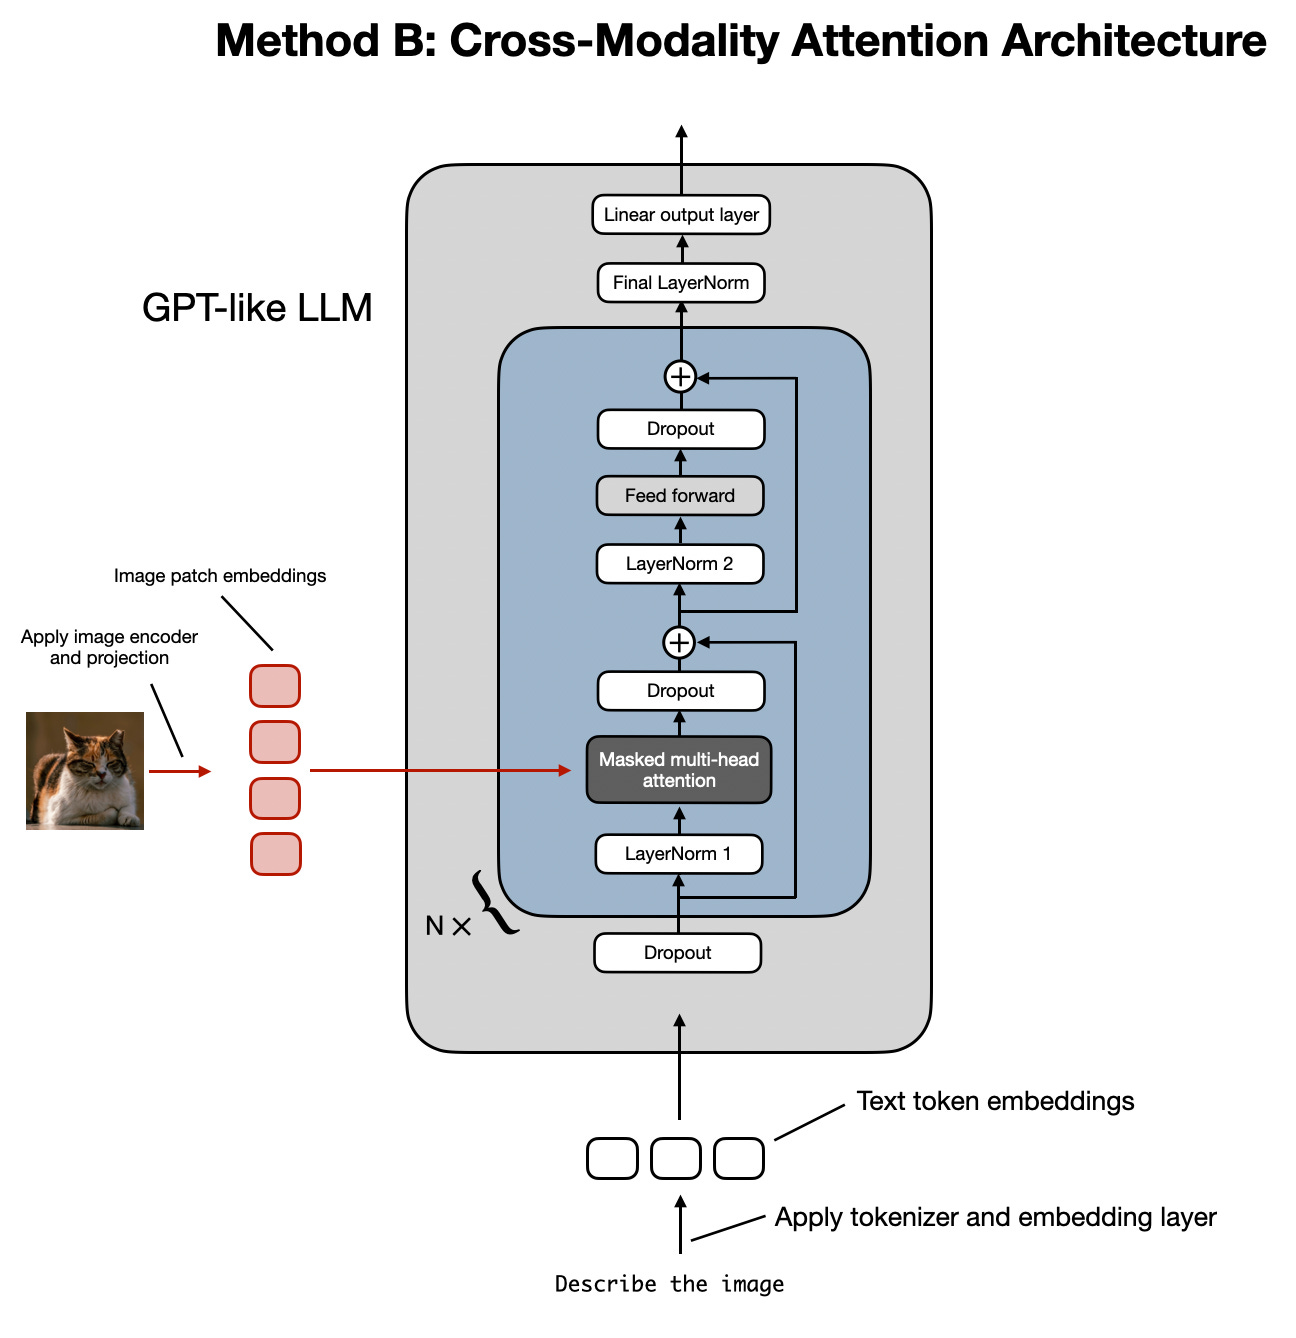
\includegraphics[width=0.85\textwidth]{img/pdz/17-cross-attention.jpg}
    \caption[Cross-attention]{Cross-attention}
    \label{fig:Cross-attention}
\end{figure}

Cross-attention uses the same attention mechanism defined in Section~\ref{sec:transformer} (Equation~\ref{eq:attention}), but with a key difference: queries come from one sequence (the target modality, e.g., decoder text embeddings) while keys and values come from a different sequence (the source modality, e.g., encoder speech/image features). This allows the model to attend across different modalities or sequences, enabling information flow from source to target. 

Formally, for cross-attention:

\begin{itemize}
    \item $Q \in \mathbb{R}^{T_q \times d}$ are queries from the target modality (e.g., decoder text embeddings);
    \item $K, V \in \mathbb{R}^{T_k \times d}$ are keys and values from the source modality (e.g., encoder speech/image features);
    \item $d_k$ is the dimension of the key vectors;
    \item $T_q, T_k$ are token lengths for target and source sequences.
\end{itemize}

Multimodal fusion via dual attention for two modalities $A$ and $B$, cross-attention is computed independently:

\[
    H_{A} = \text{Attention}(Q, K_{A}, V_{A});
    H_{B} = \text{Attention}(Q, K_{B}, V_{B}).
\]

The fused representation is then computed as

\begin{equation*}
    H = \alpha H_{A} + (1 - \alpha)H_{B}
\end{equation*}

where $0 \leq \alpha \leq 1$ is a learnable fusion coefficient.


\section{Multimodal Embedding}

Multimodal embeddings represent heterogeneous inputs in a shared space for cross-modal retrieval. CLIP established a strong baseline by jointly training image and text encoders on large-scale paired data, enabling zero-shot image--text retrieval and serving as a backbone for later systems~\cite{radford2021clip}.



Each input modality $m \in \{\text{text}, \text{audio}, \text{vision}\}$ is encoded into a latent vector using a modality-specific encoder
\begin{equation*}
    z_m = f_m(x_m; \theta_m)
\end{equation*}
where $x_m$ is the raw input of modality $m$, $f_m(\cdot)$ is the corresponding encoder (e.g., Transformer encoder for text, Conformer for audio, ViT for vision), and $\theta_m$ denotes its learnable parameters. An example of multimodal embedding is shown in Figure~\ref{fig:Multimodal embedding}\footnote{\url{https://newsletter.theaiedge.io/p/how-to-build-a-multimodal-rag-pipeline-8d6}}.

\begin{figure}[H]
    \centering
    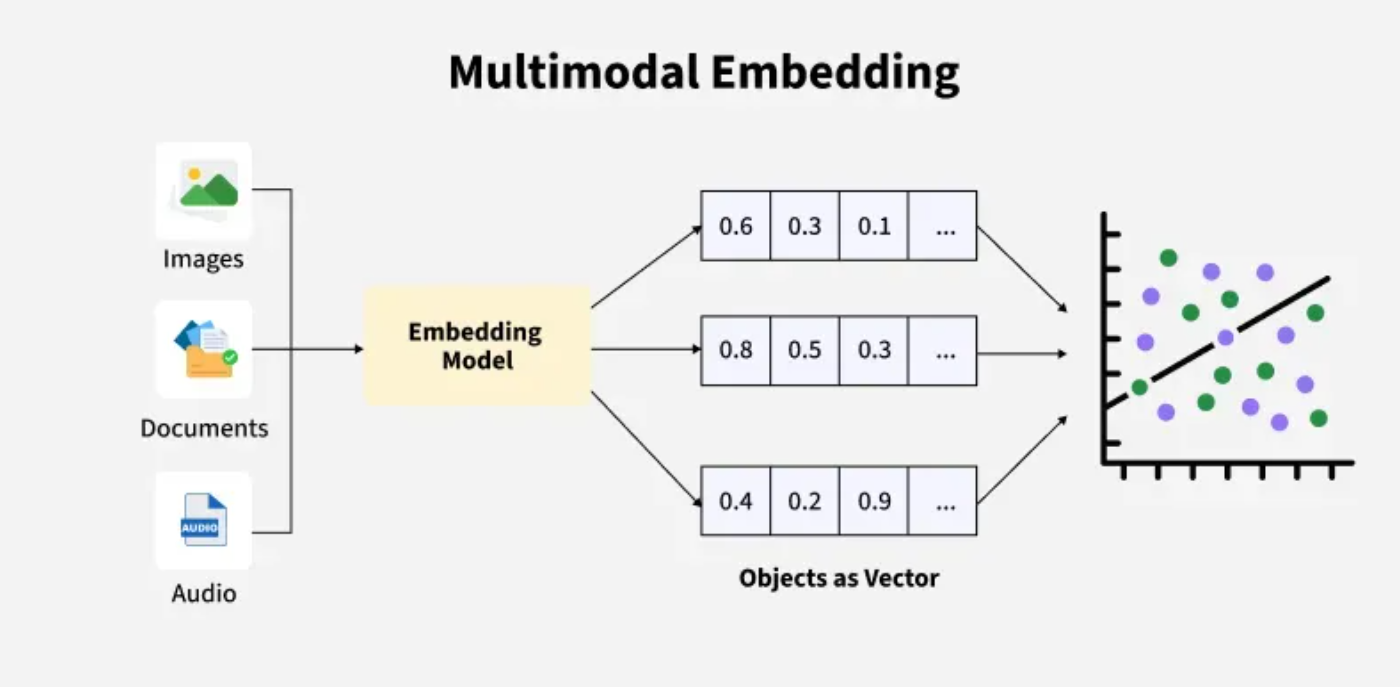
\includegraphics[width=0.9\textwidth]{img/pdz/05-multimodal-embedding.png}
    \caption[Multimodal embedding]{Multimodal embedding}
    \label{fig:Multimodal embedding}
\end{figure}


We fuse modality embeddings into a shared representation
\begin{equation*}
    z = g([z_{\text{text}}; z_{\text{audio}}; z_{\text{vision}}]; \phi)
\end{equation*}
where $[z_{\text{text}}; z_{\text{audio}}; z_{\text{vision}}]$ is the concatenation operator, $g([z_{\text{text}}; z_{\text{audio}}; z_{\text{vision}}])$ is a fusion network (e.g., MLP or cross-attention module), and $\phi$ denotes fusion parameters.

To align representations across modalities, we apply a contrastive loss
\begin{equation*}
    \mathcal{L}_{\text{contrast}} = -\sum_{i=1}^{N} \log
    \frac{\exp(\mathrm{sim}(z_i^{(a)}, z_i^{(t)}) / \tau)}
    {\sum_{j=1}^{N} \exp(\mathrm{sim}(z_i^{(a)}, z_j^{(t)}) / \tau)}
\end{equation*}
where $z_i^{(a)}$ and $z_i^{(t)}$ are the audio and text embeddings of paired sample $i$, $\mathrm{sim}(z_i^{(a)}, z_j^{(t)})$ is a similarity function (e.g., cosine similarity), $\tau$ is the temperature scaling factor, and $N$ is the batch size.


Recent work repurposes multimodal LLMs as retrievers. MM-Embed fine-tunes a multimodal LLM as a bi-encoder for image-text queries and uses modality-aware hard negatives to reduce modality bias, improving performance on M-BEIR and text retrieval benchmarks~\cite{lin2024mmembed}.

Unified embedding models extend this idea beyond image and text. ImageBind aligns images, video, text, audio, depth, thermal data, and IMU signals in one space without requiring every modality pair to be explicitly annotated~\cite{girdhar2023imagebind}. This supports educational retrieval where speech, slides, images, and video should be searchable together.

Domain-specific models target visually rich documents such as slides, tables, diagrams, and formulas. For example, jina-embeddings-v4 supports text-image retrieval, single-vector embeddings, multi-vector late interaction, and task adapters, with strong results on visually dense retrieval benchmarks such as Jina-VDR~\cite{guenther2025jinaembeddingsv4}.

Industry systems also focus on interleaved documents such as PDFs and slides. Nomic's Embed Multimodal 7B embeds mixed text-image document structures for RAG over visually rich files\footnote{\url{https://www.nomic.ai/blog/posts/nomic-embed-multimodal}}.

Overall, the gap between multimodal and single-modal retrieval is narrowing. Multimodal training can improve semantic representations even for text-only tasks, which is valuable in educational settings where queries often combine textual and visual references.

\textbf{Simplified Overview of Multimodal Embedding Models}

The following table provides a concise summary of the landmark multimodal embedding models discussed in this section, highlighting their architectural focus and primary strengths for educational RAG applications.

\begin{table}[H]
\centering
\caption{Comparison of Multimodal Embedding Models}
\label{tab:multimodal_models_overview}
\scalebox{0.85}{
\begin{tabular}{lp{3cm}p{5cm}p{4cm}}
\toprule
\textbf{Model} & \textbf{Modalities} & \textbf{Key Innovation} & \textbf{Primary Use Case} \\ \midrule
\textbf{CLIP} & Image, Text & Joint contrastive pre-training on 400M pairs. & Baseline cross-modal alignment. \\
\textbf{MM-Embed} & Image, Text & Modality-aware hard negatives to reduce text bias. & Balanced multi-domain retrieval. \\
\textbf{ImageBind} & 6 Modalities & Unified embedding space for Text, Image, Audio, etc. & Cross-modal search (e.g., Audio $\rightarrow$ Image). \\
\textbf{Jina-v4} & Image, Text & Task-specific LoRA adapters and late-interaction. & Visually rich documents (slides, tables). \\
\textbf{Nomic 7B} & Interleaved & Native support for interleaved document structures. & Multi-page PDF/Slide RAG. \\ \bottomrule
\end{tabular}
}
\end{table}

\section{RAG}

\subsection{Historical Evolution of RAG}

\textbf{2017--2019: Pre-RAG foundations.}
Before RAG, open-domain QA commonly used retrieve-then-read pipelines: a sparse retriever fetched passages and a neural reader extracted answers. DrQA established this pattern with TF-IDF/BM25 retrieval and neural reading~\cite{chen2017drqa}. ORQA then showed that dense retrievers could be trained from QA supervision~\cite{orqa2019}, while kNN-LMs demonstrated inference-time access to external datastores~\cite{khandelwal2020knnlm}.

\textbf{2020: Formalizing RAG.}
REALM introduced differentiable retrieval during language-model pretraining, showing that an LM could consult updateable external knowledge~\cite{realm2020}. RAG then combined DPR retrieval with a BART generator and trained the retriever-generator system for knowledge-intensive tasks~\cite{lewis2020rag}.

\textbf{2021--2022: Stronger Retrievers, Multi-Document Reasoning, and Lighter Readers.}
This period improved retrieval, evidence fusion, and query reformulation. RocketQA, RocketQAv2, Condenser, Contriever, and GTR strengthened dense retrieval through hard negatives, distillation, retriever-oriented pretraining, unsupervised contrastive learning, and scaling~\cite{rocketqa2021, rocketqa2_2021, condenser2021, contriever2021, gtr2021}. ColBERTv2 made late-interaction retrieval more practical, while SPLADE showed the value of learned sparse representations and hybrid fusion~\cite{colbertv2_2021, splade2021, formal2021splade}. Multi-document systems such as EMDR, MDR, FiD, KG-FiD, FiD-Light, and RETRO improved multi-hop evidence use and semi-parametric generation~\cite{emdr2021, mdr2020, fid2020, kgfid2021, fidlight2022, retro2021}. Query reformulation methods such as GAR, Self-Ask, ReAct, WebGPT, and HyDE became reusable components for improving first-stage recall and reasoning~\cite{gar2021, selfask2022, react2022, webgpt2021, hyde2022}.

\textbf{2023--2024: From fixed pipelines to adaptive, verifiable, and structure-aware systems.}
Recent RAG systems increasingly decide when, what, and how much to retrieve. FLARE, Adaptive-RAG, SEAKR, and DRAGIN trigger or route retrieval dynamically~\cite{flare2023, adaptive_rag2024, seakr2024, dragin2024}. SELF-RAG, CRAG, and CoV-RAG add critique, filtering, refusal, or verification to reduce unsupported generation~\cite{selfrag2023, crag2024, covrag2024, lmpriors2024}. Context compression and ranking became central through RankRAG and LLMLingua~\cite{rankrag2024, llmlingua2023, compression2024}, while GraphRAG/GRAG introduced structure-aware retrieval over entities and relationships~\cite{graphrag2024, grag2024}. LongRAG and self-routing explored how long-context LLMs and targeted retrieval can be combined~\cite{longrag2024, selfroute2024}.

\textbf{2025: Agentic control, standardized modules, faithful decoding, evaluation, and memory.}
By 2025, Agentic RAG emphasizes planning, tool use, reflection, and multi-agent control over retrieval; HopRAG is an example of graph-guided multi-hop retrieval before generation~\cite{survey_agentic2025, survey_reasoning_agentic2025, hoprag2025}. Surveys increasingly describe RAG as modular: retrieval optimization, context processing, generation optimization, and evaluation/monitoring~\cite{knowledge_oriented_survey2025, architectures_survey2025}. Faithfulness methods such as FaithfulRAG, ReCLAIM, CiteFix, and citation benchmarks focus on grounding and attribution~\cite{faithfulrag2025, reclaim2024, citefix2025, source_attribution2025, citeeval2025}. Evaluation and memory-oriented systems such as ARES, HippoRAG-2, MemoRAG, Mem0, MIRIX, and MemOS further connect RAG with monitoring, persistent memory, provenance, and continual learning~\cite{ares2024, survey_eval2025, ragtifier2025, hipporag2_2025, memorag2024, mem0_2025, mirix2025, memos2025}.

\subsection{MRAG: The Convergence}
\textbf{Pre-RAG signals for vision–language tasks.}  
Before MRAG was named, factual VQA exposed the limits of image-only reasoning. “Straight to the Facts” explicitly learned KB retrieval for VQA, and OK-VQA required outside knowledge, catalyzing retrieval-style VQA where images must be grounded in world facts \cite{marino2019okvqa}.

\textbf{2022–2023: Early MRAG patterns.}  
Early MRAG combined VQA-style retrieval with cross-modal embeddings. TRiG converted images into text, retrieved passages, and answered in natural-language space~\cite{gao2022trig}, while entity-focused dense retrieval improved OK-VQA retrieval~\cite{wu2022entityvqa}. CLIP/ALIGN supplied shared image-text spaces, and REVEAL connected retrieval and generation during visual-language pretraining with multimodal memory~\cite{hu2023reveal}. Most systems still retrieved textual evidence such as captions, OCR, or Wikipedia, then fused it into a VL encoder/decoder.

\textbf{2024: Maturation – better retrieval and fusion for VLMs, and broader modality bindings.}  
VisRAG treats visually rich documents as first-class evidence by combining OCR text with visual region cues~\cite{yu2024visrag}. RAVEN frames retrieval-augmented VLM fine-tuning as a general recipe~\cite{rao2024raven}, while ImageBind supports one shared embedding space across six modalities, motivating unified MRAG indexes for heterogeneous educational assets~\cite{girdhar2023imagebind}.

\textbf{2025: Advanced MRAG – domains, video, documents, and built-in retrieval.}  
Recent MRAG work expands into domain-specific and video/document settings. RS-RAG integrates satellite imagery with world knowledge for remote sensing tasks~\cite{wen2025rsrag}, while unified MRAG systems combine text, image, table, and video evidence in one pipeline~\cite{drushchak2025unified}. Surveys report that MRAG improves grounding and reduces hallucinations for visually grounded queries compared with text-only RAG~\cite{mei2025survey}.



\subsection{Pipeline}

A MRAG pipeline is illustrated in Figure~\ref{fig:MRAG pipeline}\footnote{\url{https://newsletter.theaiedge.io/p/how-to-build-a-multimodal-rag-pipeline-8d6}}.

\begin{figure}[H]
    \centering
    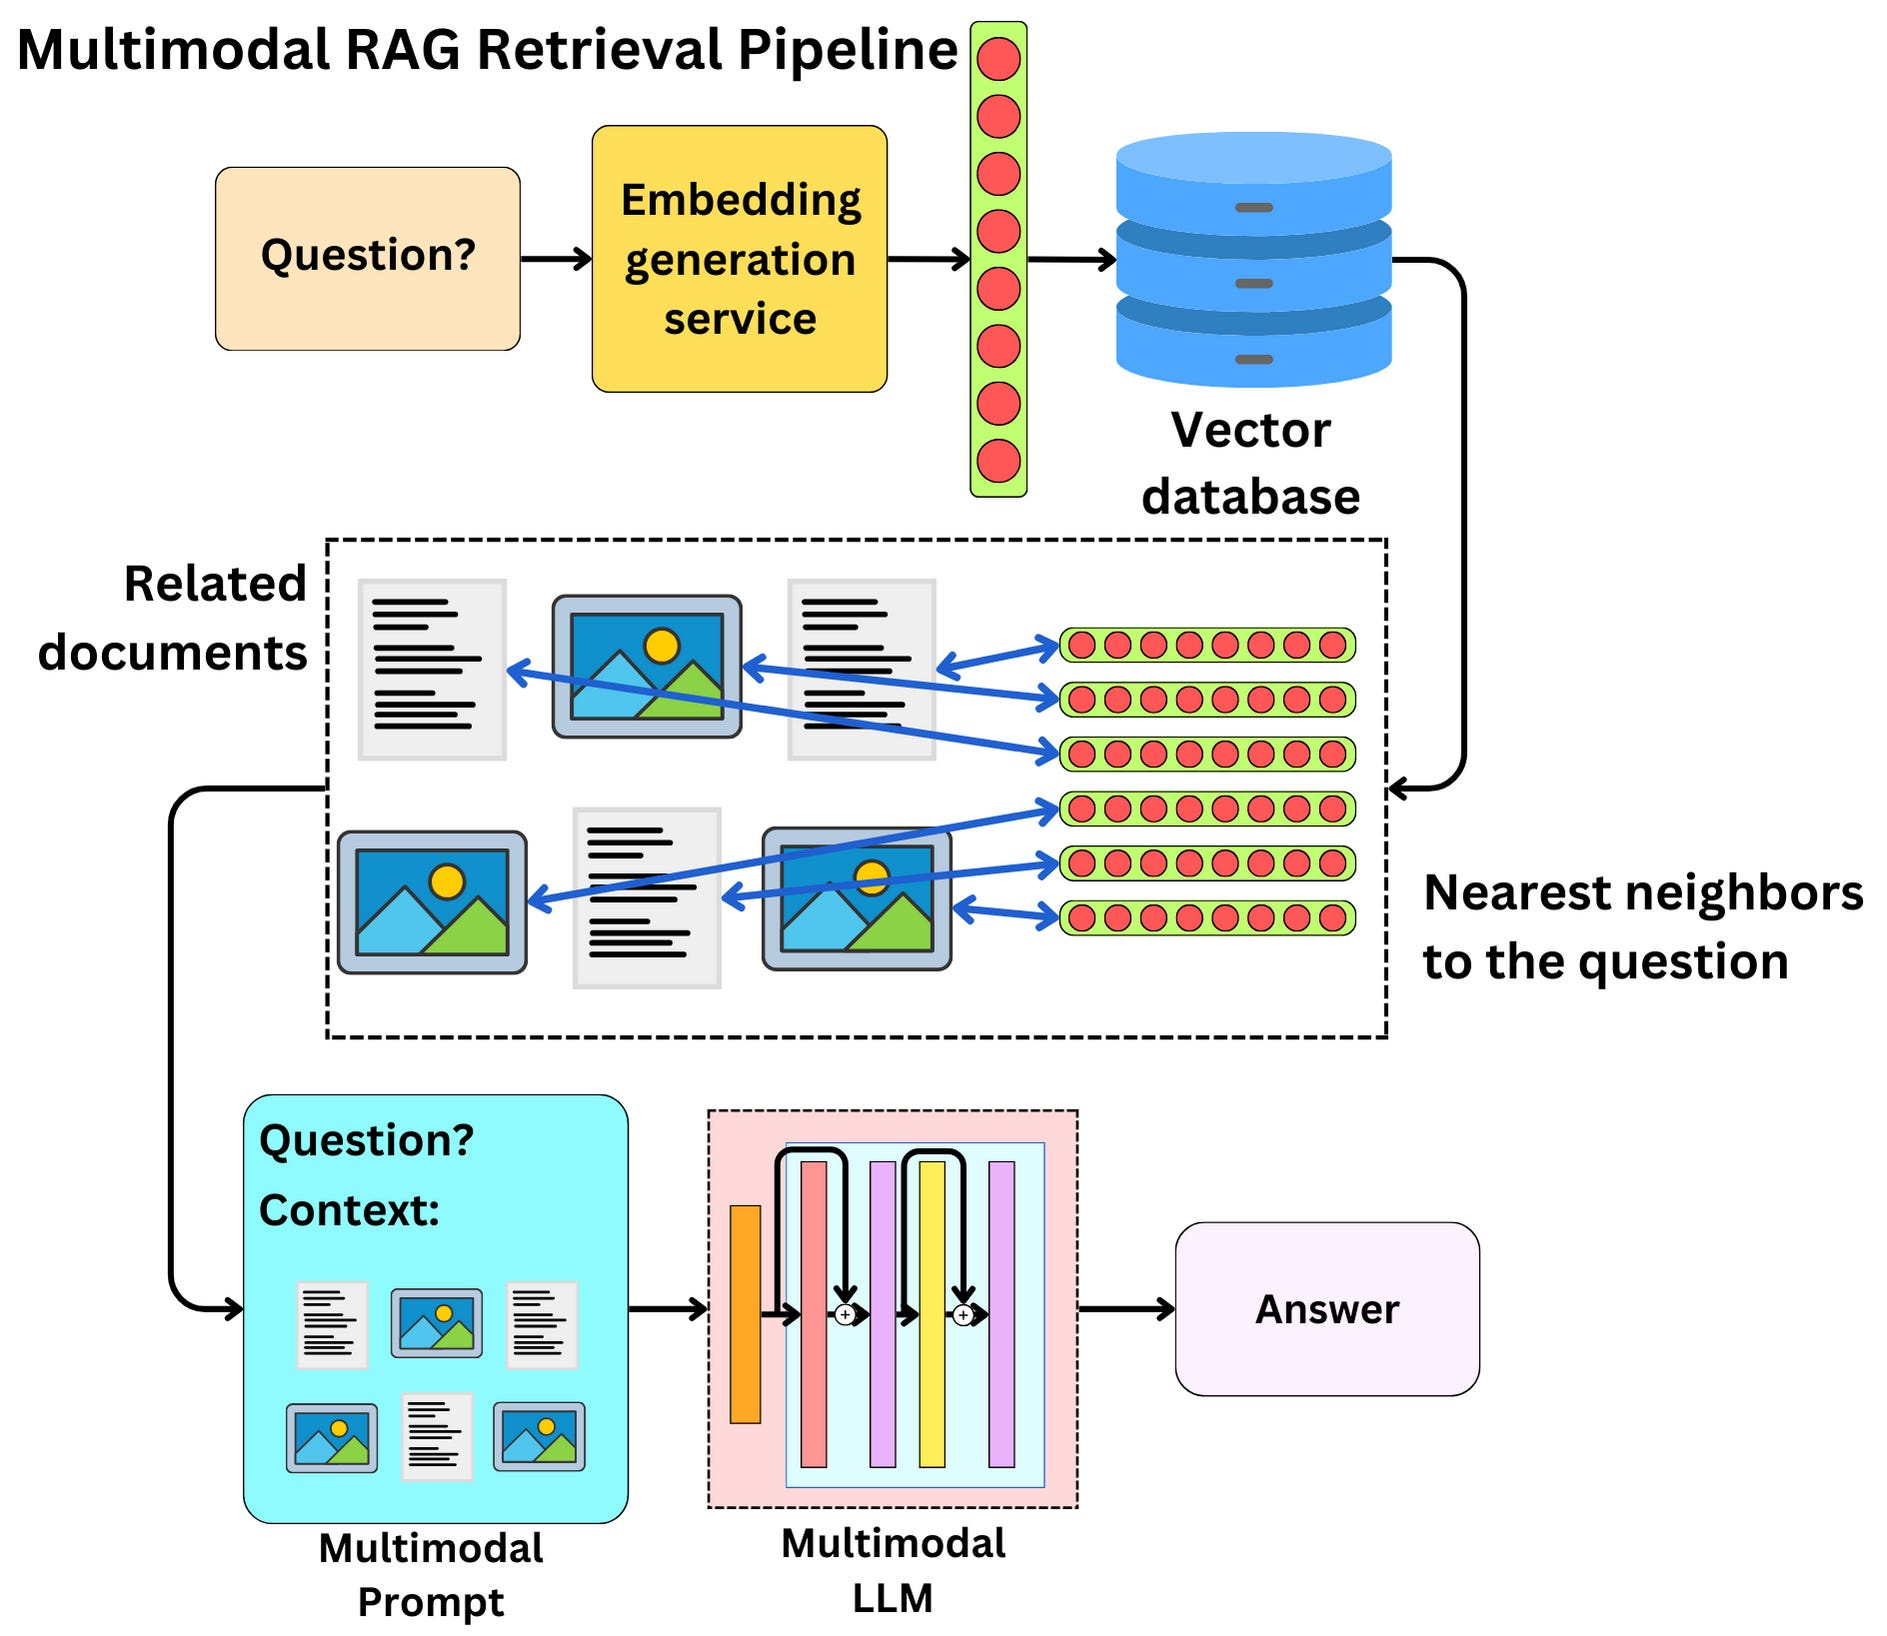
\includegraphics[width=0.9\textwidth]{img/pdz/02-multimodal-rag-pipeline.jpg}
    \caption[MRAG pipeline]{MRAG pipeline}
    \label{fig:MRAG pipeline}
\end{figure}

The pipeline combines retrieval with generation to produce grounded answers. A query is encoded into a vector representation, matched against a pre-indexed Vector Database, and used to retrieve relevant documents or passages~\cite{karpukhin2020dense, lewis2020rag}. Retrieved evidence may then be filtered, summarized, or restructured before being passed to the LLM context~\cite{izacard2021leveraging}.

RAG has two core modules: a retriever and a generator. The retriever searches external knowledge using sparse, dense, hybrid, or neural methods~\cite{lewis2020rag, luan2021sparse_dense}; the generator conditions on both the user query and retrieved context to produce the answer~\cite{izacard2022rag_sequence}. This design improves factual grounding and enables access to domain-specific or updated knowledge without retraining the language model~\cite{izacard2021leveraging, gao2023rag_survey}.

MRAG extends this pipeline to text, image, video, table, and graph evidence. Recent systems explore modality-aware retrieval, reranking, multi-agent retrieval, and reflective generation to improve answer quality in visually rich and knowledge-intensive tasks~\cite{hu2025mrag, liu2025hmrag, zhang2024mr2ag}.

\subsection{Retrieval}

Sparse retrieval maps text into high-dimensional lexical vectors~\cite{robertson2009probabilistic, formal2021splade}. Methods such as TF-IDF, \textbf{BM25}, and SPLADE are efficient and interpretable for exact keyword matching, usually implemented with inverted indexes. Their limitation is lexical mismatch: relevant documents may be missed when they use different wording from the query.
% The \textbf{BM25} algorithm is illustrated in Figure~\ref{fig:BM25}\footnote{\url{https://www.geeksforgeeks.org/what-is-bm25-best-matching-25-algorithm/}}.

% \begin{figure}[H]
%     \centering
%     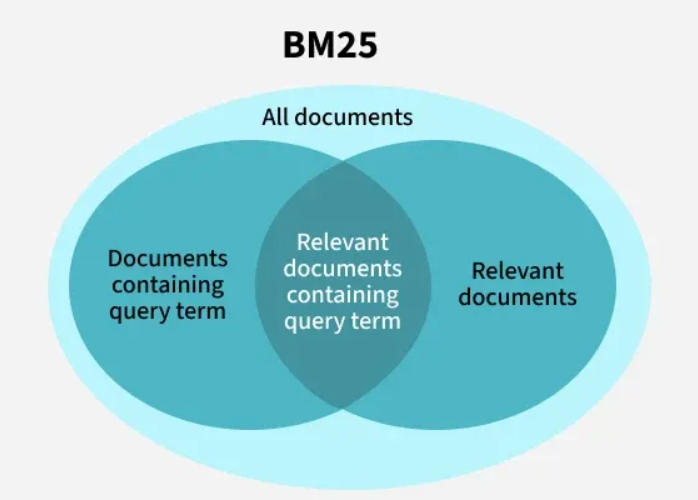
\includegraphics[width=0.6\textwidth]{img/pdz/16-bm25.png}
%     \caption[BM25]{BM25}
%     \label{fig:BM25}
% \end{figure}


Dense retrieval uses neural encoders to map queries and documents into a shared embedding space where semantic similarity is measured by vector proximity~\cite{karpukhin2020dense}. Dual-encoder models such as DPR and SPECTER2 can retrieve semantically related content even when keywords differ~\cite{singh2022scirepeval}. Large-scale dense retrieval typically relies on Approximate Nearest Neighbor Search, including HNSW indexes~\cite{malkov2016efficient}. However, dense vectors can be weaker on exact term matching and may lose detail in long documents~\cite{formal2021splade}.

Hybrid retrieval combines sparse and dense signals to improve robustness in RAG systems~\cite{lewis2020rag, formal2021splade, karpukhin2020dense}. Common strategies include score fusion, merging separate sparse/dense result lists, or building unified hybrid indexes. Key challenges are score calibration, distribution mismatch, and the computational cost of high-dimensional sparse vectors; distribution alignment and adaptive two-stage search can help balance accuracy and speed~\cite{iida2022unsupervised}.

Once embeddings have been generated, the retrieval module identifies and returns the most relevant
documents for a given query. In a RAG pipeline, this step is essential because it supplies the language
model with context that guides accurate response generation. Formally, given a query $q$ in language $x$,
the retriever returns a document $d$ in language $y$ (which may or may not match $x$) from a corpus
$D_y$. The retrieval function $f_n^\ast$ may be implemented using dense, lexical, or multi-vector retrieval
methods~\cite{chen2024bge}
\[
    d_y \leftarrow f_n^\ast(q_x, D_y).
\]

\textbf{Dense Retrieval:} A query $q$ is encoded into hidden states $H_q$ using a text encoder. The representation of the query
is the normalized hidden state of the special token \texttt{[CLS]}
\[
    e_q = \mathrm{norm}(H_q[0]).
\]
Similarly, for a passage $p$
\[
    e_p = \mathrm{norm}(H_p[0]).
\]
Relevance is computed as the inner product
\[
    s_{\mathrm{dense}} = \langle e_p, e_q \rangle.
\]

\textbf{Lexical Retrieval:} For each term $t$ in the query
\[
    w_{q t} = \mathrm{ReLU}(W_{\mathrm{lex}}^\top H_q[i]),
\]
and similarly for a passage
\[
    w_{p t} = \mathrm{ReLU}(W_{\mathrm{lex}}^\top H_p[i])
\]
where
\[
    W_{\mathrm{lex}} \in \mathbb{R}^{d \times 1};
\qquad
\mathrm{ReLU}(x) = \max(0, x).
\]

\textbf{Multi-vector Retrieval:} Both queries and passages are represented using multiple vectors.

\[
    E_q = \mathrm{norm}(W_{\mathrm{mul}}^\top H_q),
    \qquad
    E_p = \mathrm{norm}(W_{\mathrm{mul}}^\top H_p),
\]
where
\[
    W_{\mathrm{mul}} \in \mathbb{R}^{d \times d},
\]
and the normalization function is applied column-wise.


\subsection{Rerankers}

Rerankers, commonly implemented as cross-encoders, refine search results by jointly encoding a query--document pair to compute a relevance score. Unlike bi-encoders, which independently embed queries and documents into fixed-length vectors, rerankers leverage full token-level interactions, enabling more precise semantic matching. They are typically integrated into two-stage retrieval pipelines, where the first-stage retriever generates candidate documents and the reranker refines their ordering to achieve higher accuracy. The reranking process is illustrated in Figure~\ref{fig:Reranker}\footnote{\url{https://www.together.ai/blog/together-rerank-api-and-salesforce-llamarank}}.

\begin{figure}[H]
    \centering
    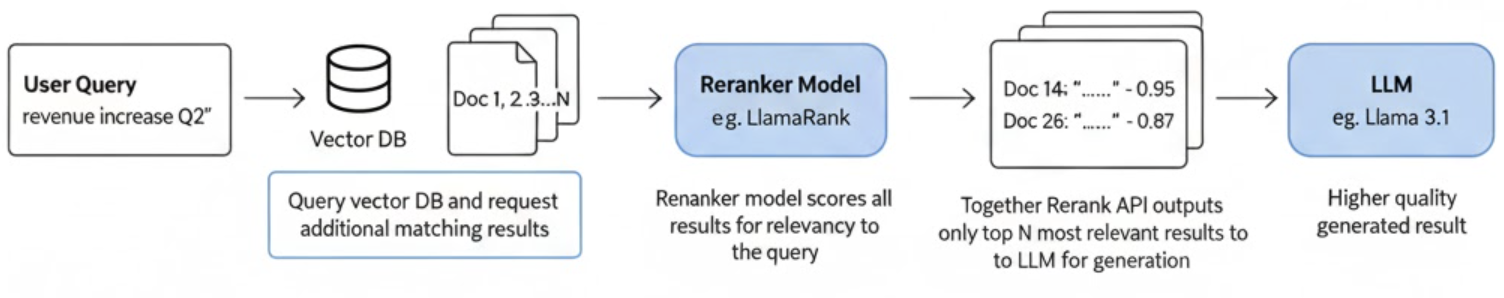
\includegraphics[width=1\textwidth]{img/pdz/18-reranker.png}
    \caption[Reranker]{Reranker}
    \label{fig:Reranker}
\end{figure}

Rerankers model token-level cross-attention between the query and document, which improves precision for entity matching, negation, semantic alignment, factual verification, and multi-hop reasoning.

Rerankers are computationally expensive and therefore operate on a narrowed candidate set rather than the full corpus. This architecture is decomposed as follows:
\begin{itemize}
    \item Stage 1 (Efficient Retrieval): A bi-encoder or sparse retriever (e.g., BM25, DPR, ColBERT) selects the top-$k$ candidates efficiently using vector similarity or lexical matching.
    \item Stage 2 (Precision Reranking): A cross-encoder transformer takes $(q, d)$ jointly as input and outputs a scalar relevance score used to reorder the candidate list.
\end{itemize}

This separation balances scalability and accuracy: fast retrieval reduces search space, while rerankers optimize precision at the top ranks.


Bi-encoders compute representations independently:
\[
\text{doc} \rightarrow \mathbf{v}_d \in \mathbb{R}^d, \quad \text{query} \rightarrow \mathbf{v}_q \in \mathbb{R}^d
\]
Similarity is computed via vector metrics (e.g., dot product), which is efficient but compresses document semantics into a single vector without query-context information.

Rerankers instead compute relevance jointly. This allows the model to consider local alignments and contextual dependencies, improving performance on tasks requiring fine-grained semantic reasoning. However, the computation happens online for each query-document pair and cannot be precomputed.


Bi-encoder indexing is performed offline, so inference requires only query encoding and approximate nearest neighbor search. Rerankers require full transformer inference for every candidate document:
\[
q + d \rightarrow \text{Transformer} \rightarrow \text{score}
\]
Because this cost scales with the candidate count, rerankers are typically applied to only 10--1000 candidates rather than the full index.

\subsubsection*{Impact on Retrieval Quality}

Empirically, rerankers improve metrics such as Recall and Mean Reciprocal Rank, especially in:
\begin{itemize}
    \item open-domain question answering
    \item legal and biomedical retrieval where precision is critical
    \item multi-step reasoning and claim verification
    \item reranking passages in RAG pipelines for LLM-based generation
\end{itemize}

Token-level attention helps distinguish subtle semantic variations, such as contradiction versus support, that bi-encoders may compress away.

\begin{itemize}
    \item \textbf{Bi-encoders:} Scalable retrieval with precomputed embeddings, but limited by lossy compression.
    \item \textbf{Rerankers:} High precision via joint computation, but expensive at query time.
    \item \textbf{Two-stage retrieval:} Combines scalability and precision, forming the standard architecture for modern retrieval systems.
\end{itemize}


Neural reranking has evolved from cross-encoders over BM25 candidates to more scalable and generative approaches. ColBERT-v2 preserves token-level late interaction while using compressed embeddings and approximate search for efficiency \cite{colbertv2}. MonoT5 frames relevance as a sequence-to-sequence generation task \cite{monot5}, TART uses instruction-tuned reranking for zero-shot transfer \cite{tart}, and RankGPT applies LLMs to listwise ranking and reasoning across candidate sets \cite{rankgpt}. These trends make rerankers both precision filters and semantic evaluators in modern RAG pipelines.

\subsection{Augmentation}

The augmentation process in RAG is illustrated in Figure~\ref{fig:Augmentation}\footnote{\url{https://obot.ai/resources/learning-center/retrieval-augmented-generation/}}.

\begin{figure}[H]
    \centering
    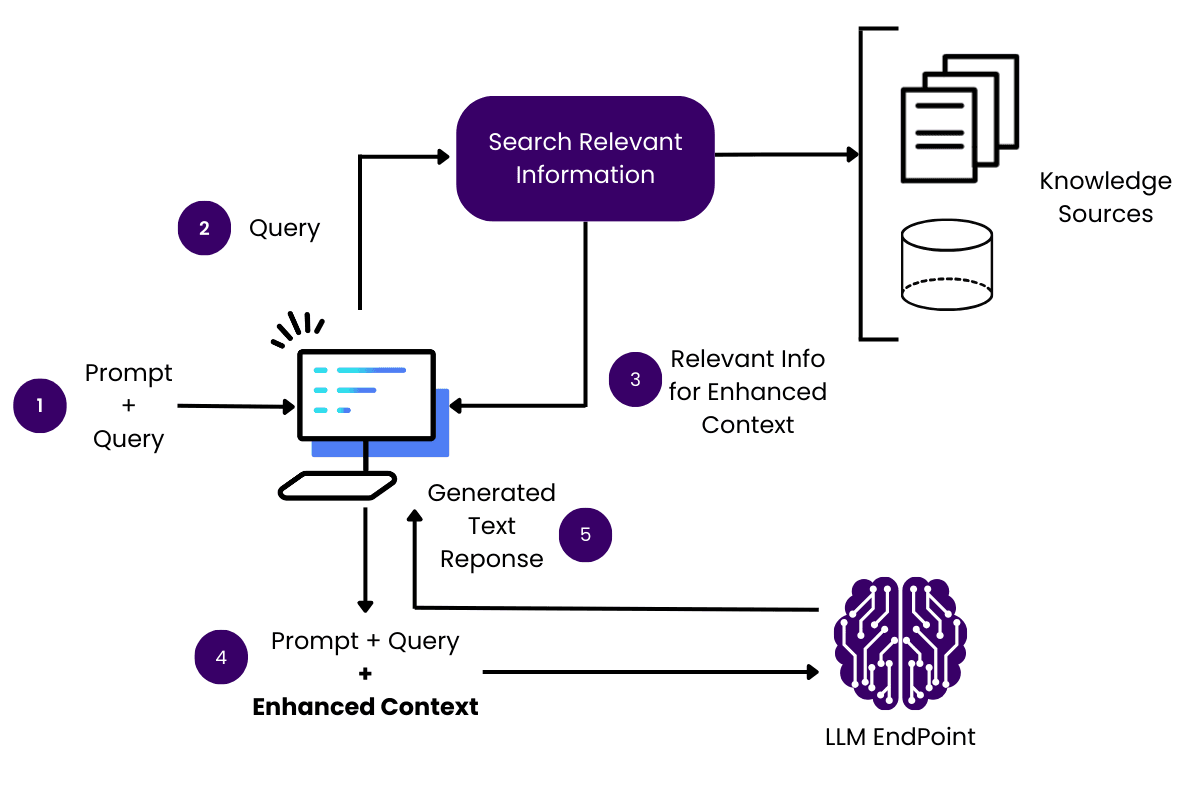
\includegraphics[width=0.9\textwidth]{img/pdz/07-augmentation.png}
    \caption[Augmentation]{Augmentation}
    \label{fig:Augmentation}
\end{figure}

Augmentation in RAG transforms retrieved knowledge before generation. It may summarize, compress, restructure, or expand evidence to improve relevance and reduce noise \cite{yoon2024compact, asai2023selfrag}.

Given a retrieved document set $D = \{d_1, \dots, d_k\}$, augmentation produces a transformed set $D' = \mathcal{A}(D)$ where $\mathcal{A}$ is an augmentation operator such as summarization, chunk merging, entity extraction, or reasoning-based synthesis. Formally:
\[
D' = \mathcal{A}(D) = \{ a_1, \dots, a_m \}, \quad m \leq k \; \text{or} \; m \geq k,
\]
where each augmented element $a_i$ may be compressed, reformatted, or newly generated from retrieval.

To preserve semantic coverage while reducing redundancy, augmentation can be framed as an optimization objective:
\[
\max_{D'} \; \text{Rel}(D', q) - \lambda \, \text{Redund}(D'),
\]
where $\text{Rel}$ measures relevance to query $q$ and $\text{Redund}$ quantifies informational overlap.

A common augmentation strategy is active document compression, where generative models summarize retrieved passages while preserving answer-critical semantics \cite{yoon2024compact}. This can be modeled as:
\[
a_i = \arg\max_{a} P(a \mid d_i, q),
\]
and scored using a utility function:
\[
s(a_i, q) = \alpha \cdot \text{Sim}(a_i, q) + \beta \cdot \text{Coverage}(a_i, d_i),
\]
where
\[
\text{Sim}(a_i, q) = \cos(g(q), h(a_i)), \quad 
\text{Coverage}(a_i, d_i) = \cos(h(a_i), h(d_i)).
\]

Augmentation also enables iterative cycles of retrieval and rewriting. Self-reflection frameworks refine evidence through reasoned critique:
\[
D^{(t+1)} = \mathcal{A}\big(D^{(t)}, y^{(t)}, c^{(t)}\big),
\]
where $y^{(t)}$ is the generated answer and $c^{(t)}$ is a critique model output guiding refinement \cite{asai2023selfrag}.

For programming tasks, retrieved demonstrations can be reformatted into template-based exemplars:
\[
a_i = \text{Format}\big(\text{Demo}(d_i)\big),
\]
supporting structural learning in applications \cite{he2024retrieval_coding}.

Thus, augmentation acts as a knowledge refinement stage that improves grounding, reduces hallucination risk, and increases domain robustness \cite{gao2023rag_survey}.


\subsection{Generation}

The generator is the synthesis module in RAG. It conditions on both the user query and retrieved evidence, improving factual grounding compared with a standalone parametric language model \cite{gao2023rag_survey}.

\begin{figure}[H]
    \centering
    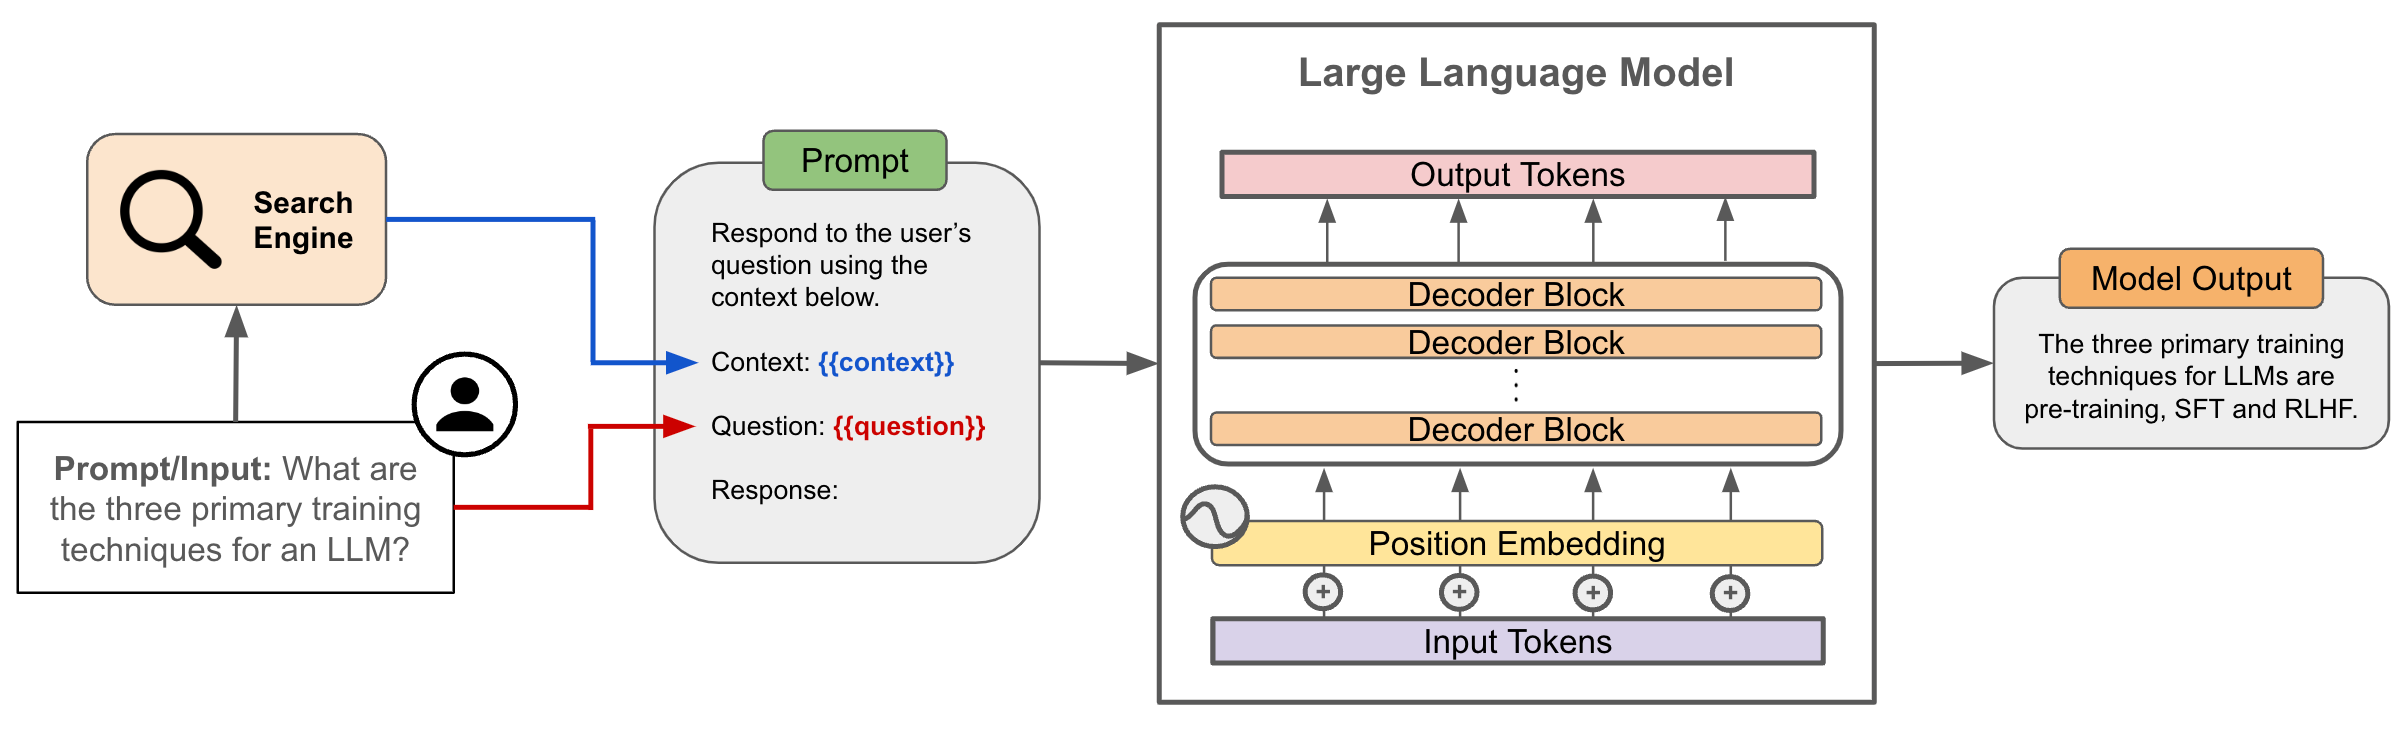
\includegraphics[width=0.9\textwidth]{img/pdz/13-generation.png}
    \caption[Generation]{Generation}
    \label{fig:Generation}
\end{figure}

Formally, given a query $q$ retrieves a document set $D = \{d_1, \dots, d_k\}$, the generator models the output sequence $y = (y_1, \dots, y_T)$ as:
\[
P(y \mid q, D) = \prod_{t=1}^{T} P(y_t \mid y_{<t}, q, D).
\]

Instead of treating retrieved documents as a single concatenated input, marginalization across documents can be applied:
\[
P(y_t \mid y_{<t}, q, D) = \sum_{d_i \in D} P(y_t \mid y_{<t}, q, d_i) \, P(d_i \mid q).
\]

Each retrieved document is encoded into a latent representation:
\[
h_i = f_{\text{enc}}(d_i),
\]
and decoding attends to these representations:
\[
P(y_t \mid y_{<t}, q, d_i) = \text{softmax}\!\left(W \cdot \text{Dec}(y_{<t}, h_i)\right).
\]

Modern RAG systems typically use autoregressive or encoder-decoder Transformers, integrating retrieved content through concatenation, cross-attention, or late fusion \cite{asai2023selfrag, yoon2024compact}.

\begin{itemize}
    \item \textbf{Concatenation-based generation:} Retrieved passages are appended to the prompt; simple but limited by context length and prone to noisy retrieval.
    \item \textbf{Cross-attention generation:} Retrieved representations act as separate attention sources to improve semantic alignment and reduce positional bias \cite{he2024retrieval_coding}.
\end{itemize}

In cross-attention generation, retrieved representations form a secondary attention memory:
\[
\text{Attention}(Q, K_D, V_D) = \text{softmax}\left(\frac{QK_D^\top}{\sqrt{d_k}}\right)V_D,
\]
where $K_D, V_D$ are keys and values derived from retrieval encodings.

\begin{itemize}
    \item \textbf{Rerank-and-generate pipelines:} Only top-ranked chunks are passed to the generator after evidence filtration \cite{zhang2024llm_hallucination_code}.
    \item \textbf{Self-reflective iterative generation:} Retrieval, generation, and critique occur recursively to enhance factual accuracy and reasoning \cite{asai2023selfrag}.
\end{itemize}

To further improve faithfulness, contrastive losses can be incorporated to prefer evidence-grounded explanations:
\[
\mathcal{L}_{\text{faith}} = -\log \frac{\exp(s(y, D^+))}{\exp(s(y, D^+)) + \exp(s(y, D^-))},
\]
where $D^+$ contains supporting evidence and $D^-$ contains retrieved distractors. The score function $s(y, D)$ measures how well a generated output $y$ is grounded in a document set $D$, commonly implemented as a similarity function such as:
\[
s(y, D) = \cos\left(g(y), \, h(D)\right),
\]
where $g(y)$ encodes the generated text and $h(D)$ aggregates document embeddings (e.g., mean pooling or attention-weighted fusion).

\subsection{Prompt Engineering}

Prompt engineering designs input prompts to control LLM behavior during inference. It steers pretrained models without modifying their parameters \cite{brown2020language}.

Core formats include \textbf{zero-shot prompting}, which uses only instructions \cite{reynolds2021prompt}, and \textbf{one-shot}/\textbf{few-shot prompting}, which add demonstrations for in-context learning \cite{brown2020language}. Reasoning-oriented methods such as \textbf{Chain-of-Thought (CoT)} elicit intermediate reasoning for multi-step tasks \cite{wei2022cot}, while self-consistency samples multiple reasoning paths to improve stability \cite{wang2023selfconsistency}.

Prompt engineering also supports \textbf{structured and reliable outputs}. Schema-based prompts can request JSON, bullet lists, or domain templates, reducing parsing failures in downstream systems\footnote{OpenAI GPT-4 Technical Report, \url{https://openai.com/research/gpt-4}}. Function calling extends this idea by constraining outputs to well-defined tool or data schemas.

Manual prompt design is heuristic and labor-intensive, so recent work explores \textbf{automated prompt optimization}. Candidate prompts can be searched and selected using validation metrics, including instruction phrasing and example ordering. Because exhaustive search is expensive, methods such as TRIPLE formulate prompt selection as a bandit problem to balance exploration and exploitation under limited query budgets \cite{shi2024triple}.

Another line treats prompts as parameters. Prefix-Tuning learns continuous soft prompts without updating model weights \cite{li2021prefix}, while AutoPrompt performs gradient-guided search over discrete trigger tokens \cite{shin2020autoprompt}. These methods improve control but may reduce interpretability.

Iterative editing methods refine human-written prompts. GrIPS applies gradient-free edits such as adding, deleting, or reordering phrases \cite{prasad2023grips}. Instruction Induction and Automatic Prompt Engineer (APE) use LLMs to generate and score candidate instructions \cite{zhou2022ape}.

OPRO further frames optimization as an LLM-driven loop: a meta-prompt stores candidate prompts and scores, and the model proposes improved prompts iteratively \cite{yao2023opro}. Such methods must control overfitting to validation data.

Reinforcement learning treats prompts as actions optimized for rewards such as validation accuracy or human preference. RLPrompt applies policy gradients to discrete prompt tokens and can improve over manual baselines, though search spaces and sparse rewards remain challenging \cite{deng2022rlprompt}.

Overall, prompt engineering has matured into a systematic methodology spanning demonstrations, reasoning scaffolds, structured outputs, and automated optimization. It remains central to reliable, controllable, and domain-aligned LLM behavior.

\newpage
